
\subsection{Pas de temps}

El pas de temps $\Delta t$ o \emph{time--step} influeix en la integració temporal. Resulta intuïtiu que, com menor sigui $\Delta t$, més precisos seran els resultats donats pel codi de simulació. Tanmateix, això depèn del problema. Per exemple, si les condicions de contorn donen lloc a gradients de temperatura importants, el flux de calor serà gran i, en conseqüència, seran necessaris $\Delta t$ petits. 

Per l'anàlisi del pas de temps s'escull una discretitació uniforme amb $N_1 = 35$\footnote{Com s'ha vist, la discretització uniforme no és la idònia pel problema actual, però d'aquesta manera els resultats dels diferents anàlisis són comparables.}. L'esquema d'integració numèrica és Crank--Nicolson, amb passos de temps $\Delta t \in {0.50, \, 1.00, \, 5.00, \, 10.00, \, 20.00, \, 50.00} \ \second$. Es calculen els mapes de temperatures en $t = 5000 \ \second$ i $t = 10000 \ \second$. La condició de covergència pel mètode de Gauss--Seidel és $\delta = 10^{-11}$. 

En la figura \ref{fig:pas_temps_5000} es mostren els mapes de temperatures en $t = 5000 \ \second$. En la figura \ref{fig:pas_temps_10000} es mostren per $t = 10000 \ \second$. Com s'aprecia, les diferències entre els diferents $\Delta t$ no són importants. Això permet treballar amb $\Delta t$ grans amb una pèrdua de precisió poc rellevant.
 
\begin{figure}[ht]
	\centering
	\begin{subfigure}{.5\textwidth}
		\centering
		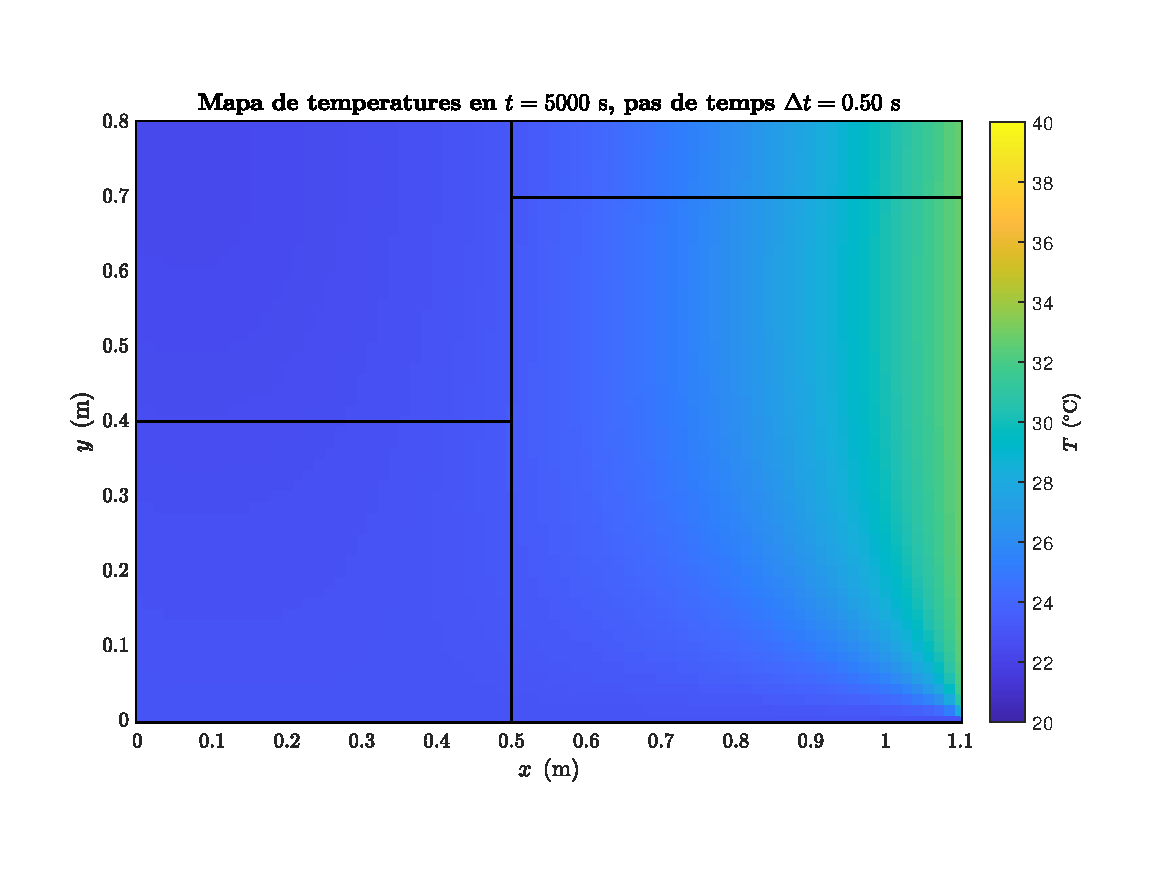
\includegraphics[width=.95\linewidth]{imagenes/04_influencia/pas_temps/pas_temps_7.pdf}
		\vspace{-15pt}
		\caption{Temps $t_\text{max} = 5000 \ \second$, pas de temps $\Delta t = 0.50 \ \second$.}
		\label{fig:pas_temps_7}
	\end{subfigure}%
	\begin{subfigure}{.5\textwidth}
		\centering
		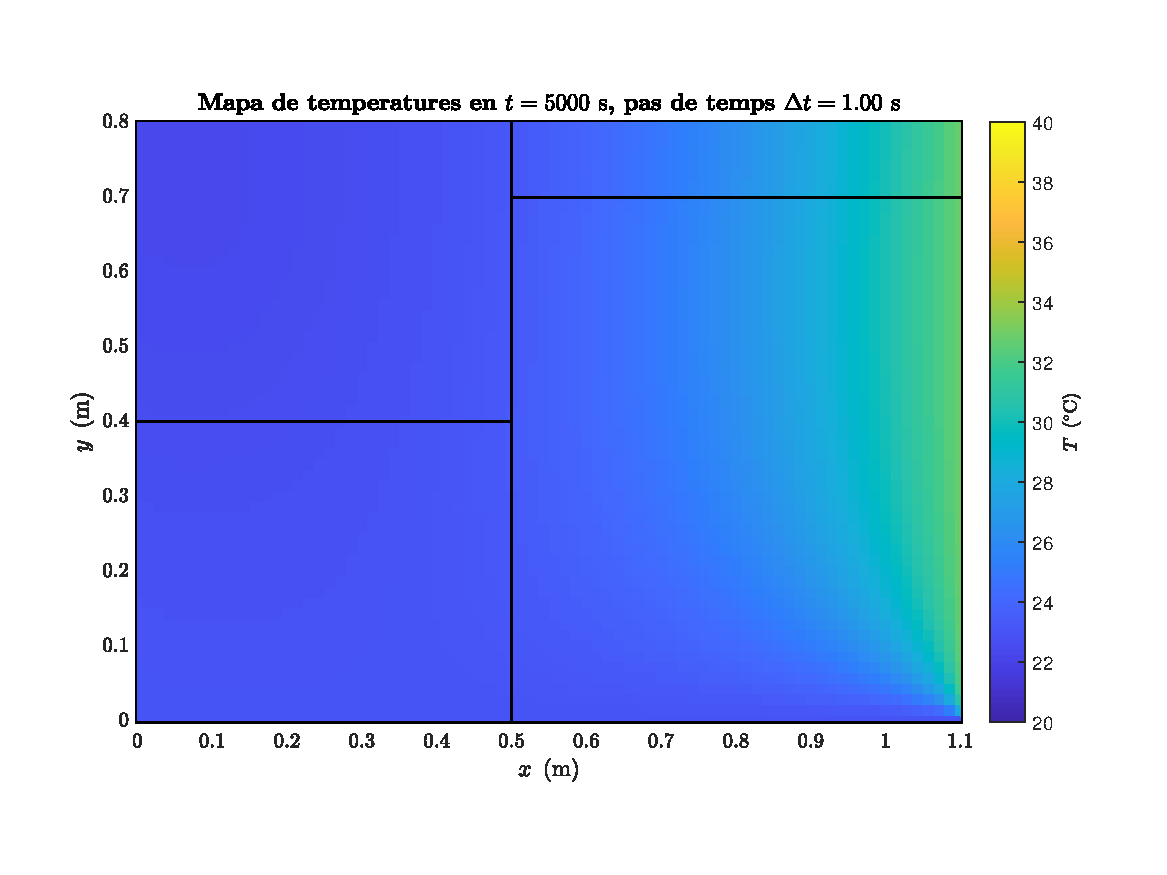
\includegraphics[width=.95\linewidth]{imagenes/04_influencia/pas_temps/pas_temps_8.pdf}
		\vspace{-15pt}
		\caption{Temps $t_\text{max} = 5000 \ \second$, pas de temps $\Delta t = 1.00 \ \second$.}
		\label{fig:pas_temps_8}
	\end{subfigure}
	\begin{subfigure}{.5\textwidth}
		\centering
		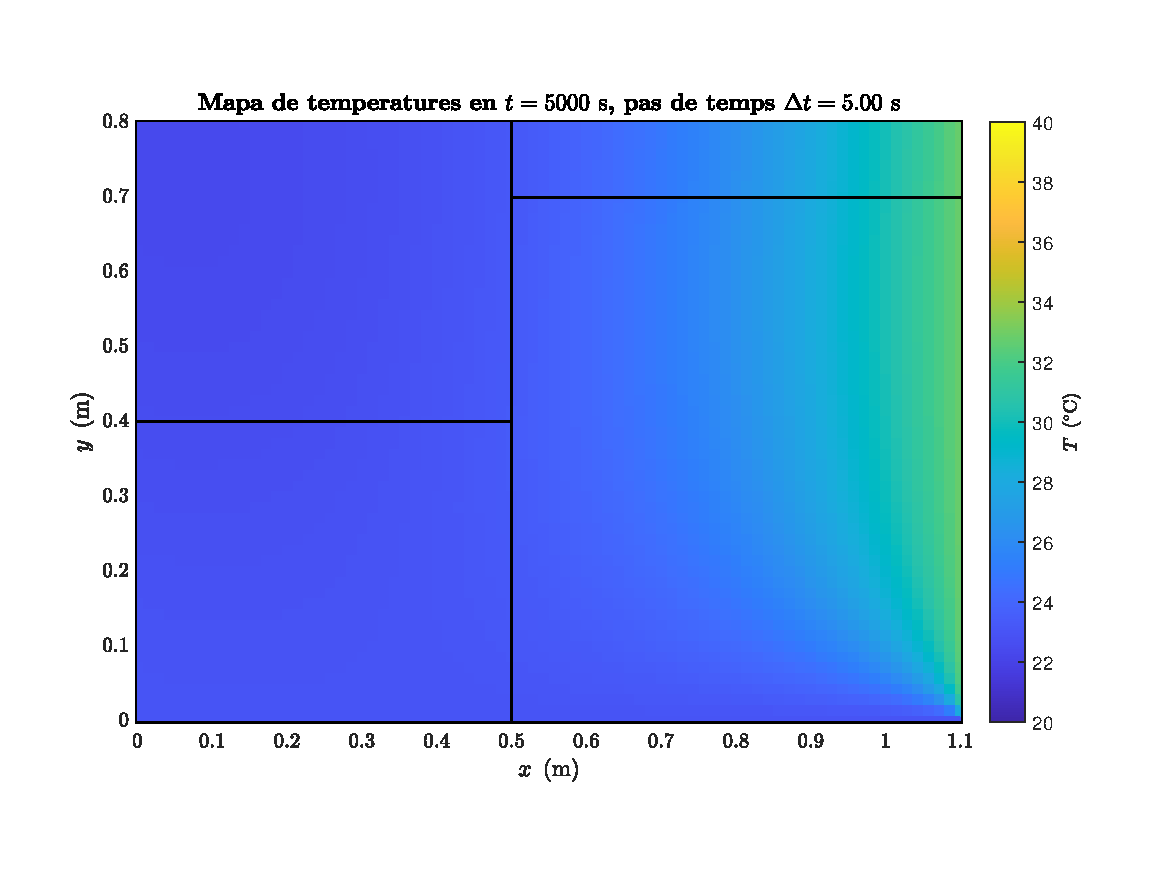
\includegraphics[width=.95\linewidth]{imagenes/04_influencia/pas_temps/pas_temps_9.pdf}
		\vspace{-15pt}
		\caption{Temps $t_\text{max} = 5000 \ \second$, pas de temps $\Delta t = 5.00 \ \second$.}
		\label{fig:pas_temps_9}
	\end{subfigure}%
	\begin{subfigure}{.5\textwidth}
		\centering
		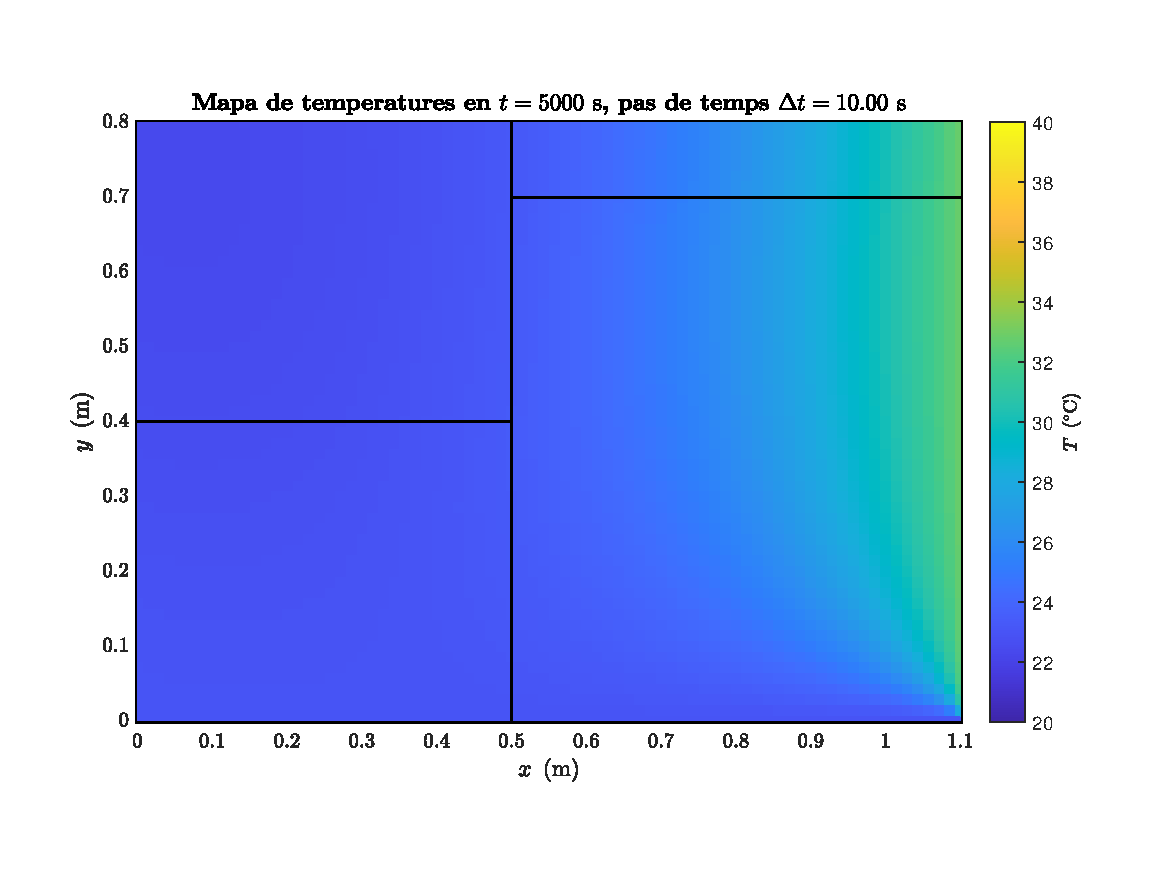
\includegraphics[width=.95\linewidth]{imagenes/04_influencia/pas_temps/pas_temps_10.pdf}
		\vspace{-15pt}
		\caption{Temps $t_\text{max} = 5000 \ \second$, pas de temps $\Delta t = 10.00 \ \second$.}
		\label{fig:pas_temps_10}
	\end{subfigure}
	\begin{subfigure}{.5\textwidth}
		\centering
		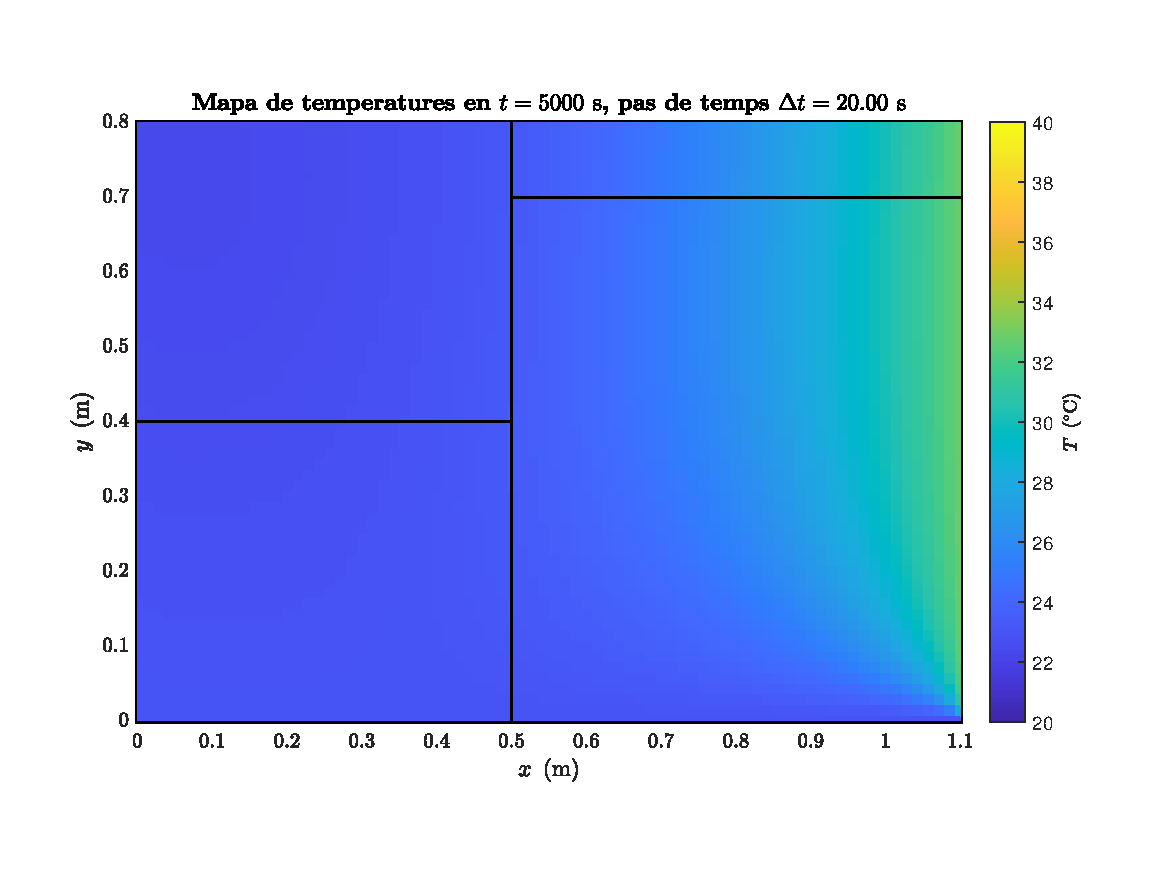
\includegraphics[width=.95\linewidth]{imagenes/04_influencia/pas_temps/pas_temps_11.pdf}
		\vspace{-15pt}
		\caption{Temps $t_\text{max} = 5000 \ \second$, pas de temps $\Delta t = 20.00 \ \second$.}
		\label{fig:pas_temps_11}
	\end{subfigure}%
	\begin{subfigure}{.5\textwidth}
		\centering
		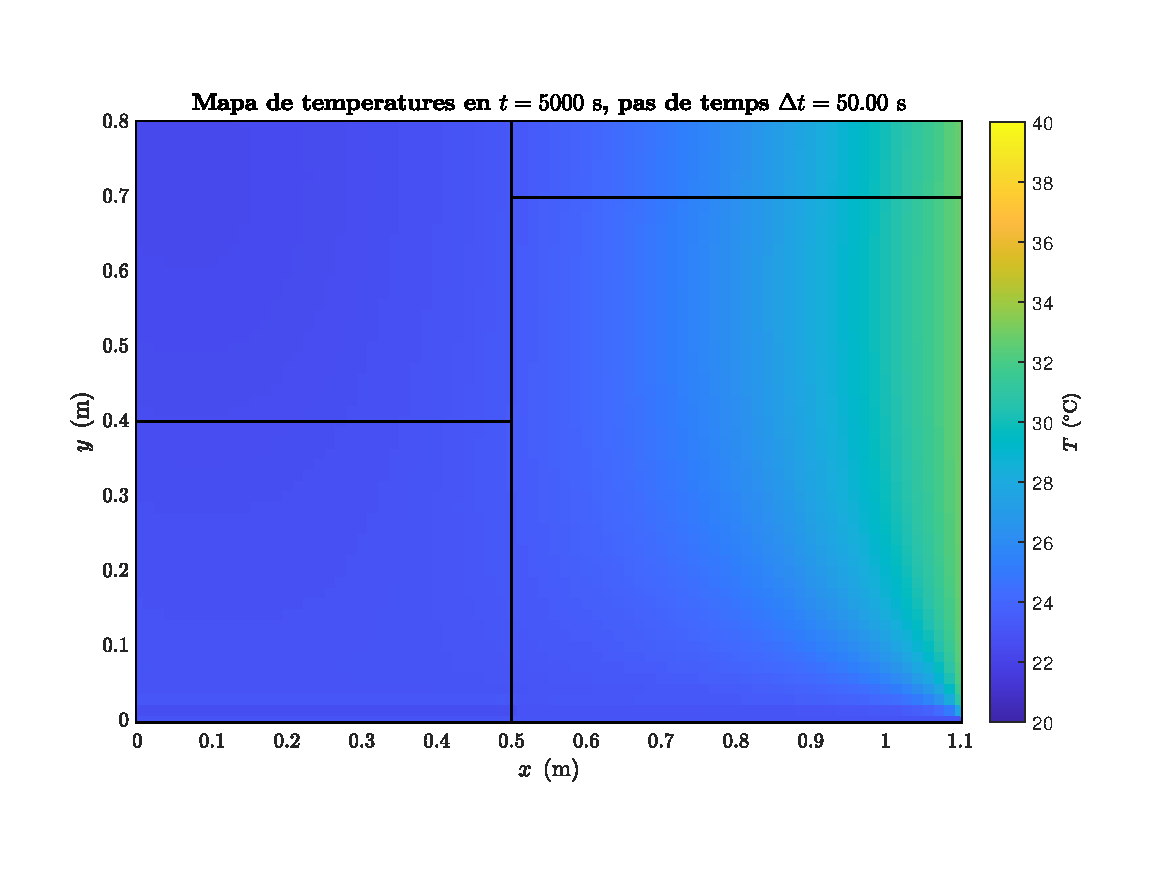
\includegraphics[width=.95\linewidth]{imagenes/04_influencia/pas_temps/pas_temps_12.pdf}
		\vspace{-15pt}
		\caption{Temps $t_\text{max} = 5000 \ \second$, pas de temps $\Delta t = 50.00 \ \second$.}
		\label{Temps fig:pas_temps_12}
	\end{subfigure}
	\caption{Mapes de temperatures en $t_\text{max} = 5000 \ \second$, discretització uniforme de $N_1 = 35$, amb passos de temps $\Delta = 0.50 \ \second, \, 1.00 \ \second, \, 5.00 \ \second, \, 10.00 \ \second, \, 20.00 \ \second$ i $50.00 \ \second,$, esquema de Crank--Nicolson i sense interpolació. L'escala de temperatures és entre $20 \ \celsius$ i $40 \ \celsius$. Com més petit és $\Delta t$, s'aprecia que la zona de major gradient tèrmic és més àmplia. A mida que $\Delta t$ creix, aquesta zona es retrau cap a la paret dreta. Més enllà d'això, no s'observen diferències significatives que indiquin que per $\Delta t = 0.50 \ \second$ s'obtinguin millors resultats que per $\Delta t = 50.00 \ \second$. Aquest fet té dues justificacions. D'una banda, l'esquema d'integració temporal és de segon ordre. D'altra banda, les propietats termofísiques i les condicions de contorn. Unes conductivitats tèrmiques més grans (\eg, $\lambda \approx 380 \ \watt / \meter \kelvin$ per l'alumini) i uns calors específics més petits, afavoririen la transferència de calor, fent necessari $\Delta t$ més petits.}	
	\label{fig:pas_temps_5000}
\end{figure} 

\begin{figure}[ht]
	\centering
	\begin{subfigure}{.5\textwidth}
		\centering
		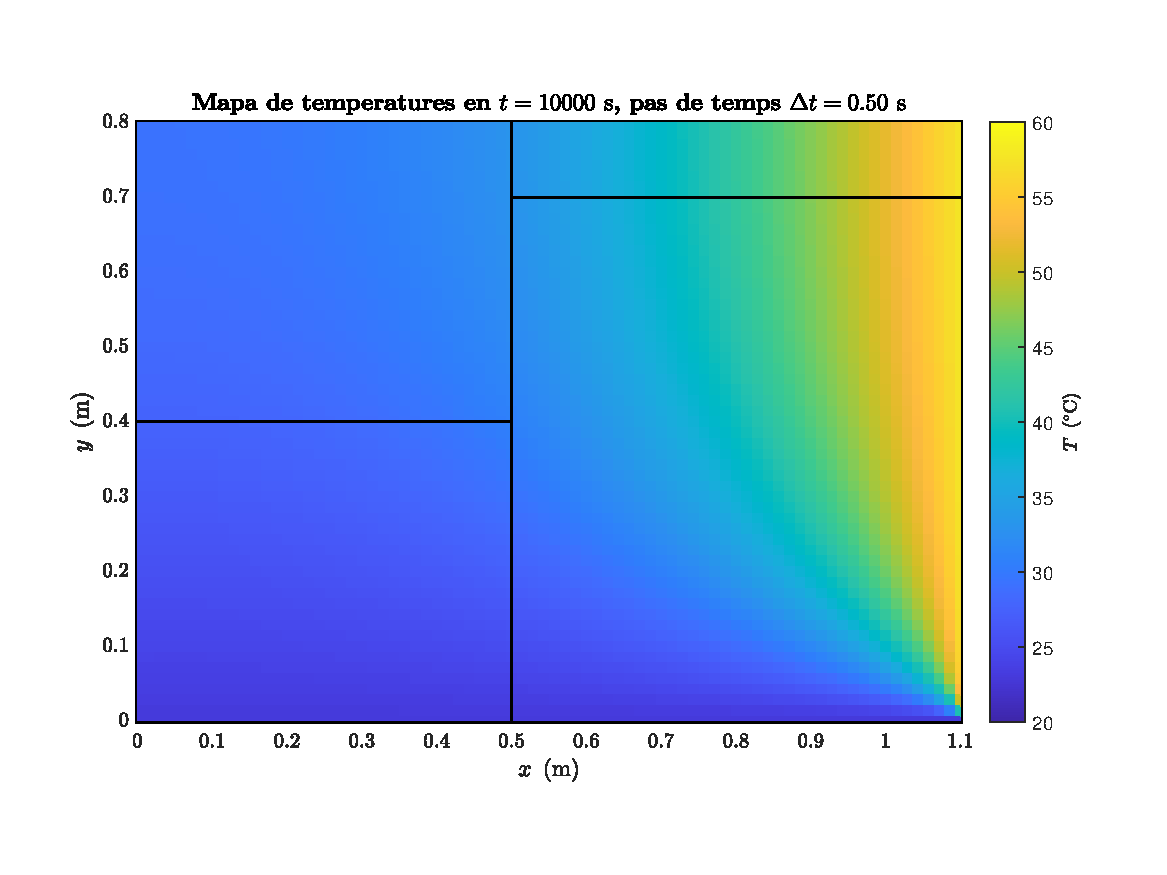
\includegraphics[width=.95\linewidth]{imagenes/04_influencia/pas_temps/pas_temps_13.pdf}
		\vspace{-15pt}
		\caption{Temps $t_\text{max} = 10000 \ \second$, pas de temps $\Delta t = 0.50 \ \second$.}
		\label{fig:pas_temps_13}
	\end{subfigure}%
	\begin{subfigure}{.5\textwidth}
		\centering
		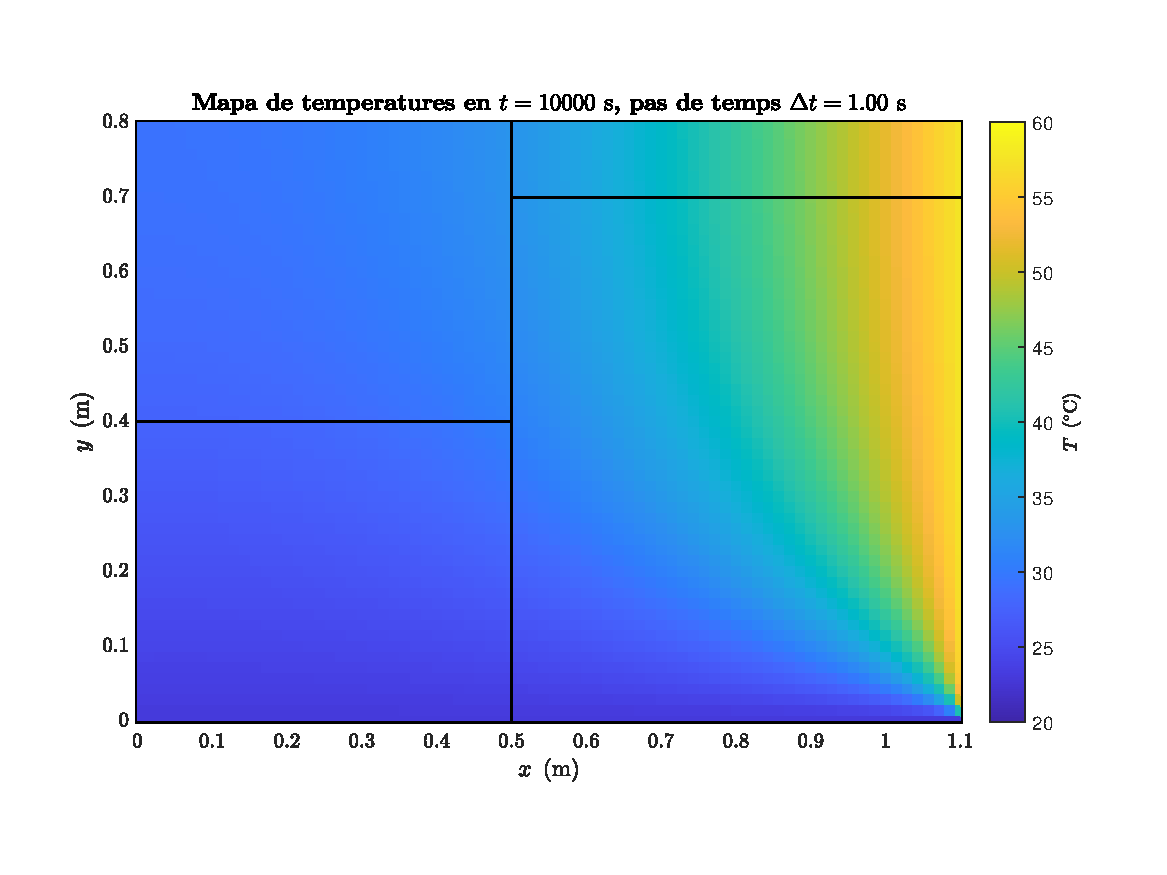
\includegraphics[width=.95\linewidth]{imagenes/04_influencia/pas_temps/pas_temps_14.pdf}
		\vspace{-15pt}
		\caption{Temps $t_\text{max} = 10000 \ \second$, pas de temps $\Delta t = 1.00 \ \second$.}
		\label{fig:pas_temps_14}
	\end{subfigure}
	\begin{subfigure}{.5\textwidth}
		\centering
		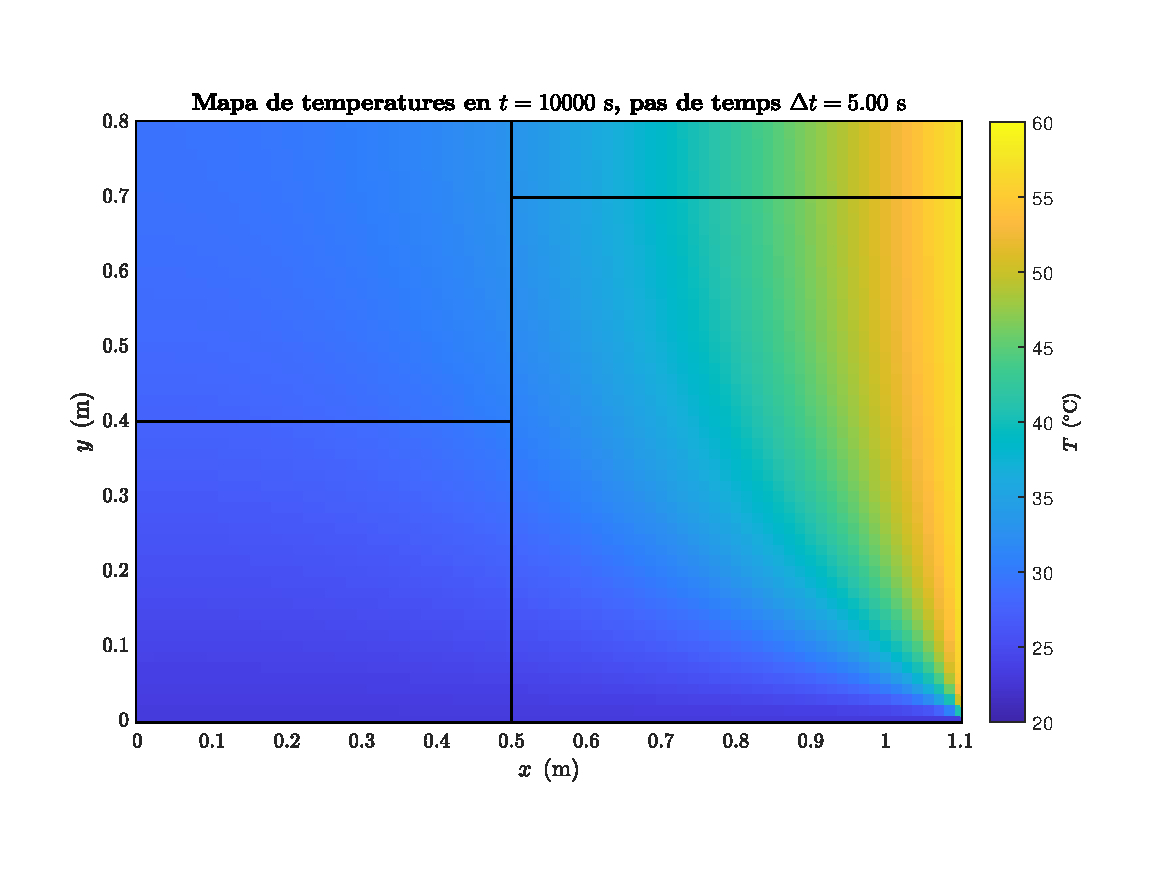
\includegraphics[width=.95\linewidth]{imagenes/04_influencia/pas_temps/pas_temps_15.pdf}
		\vspace{-15pt}
		\caption{Temps $t_\text{max} = 10000 \ \second$, pas de temps $\Delta t = 5.00 \ \second$.}
		\label{fig:pas_temps_15}
	\end{subfigure}%
	\begin{subfigure}{.5\textwidth}
		\centering
		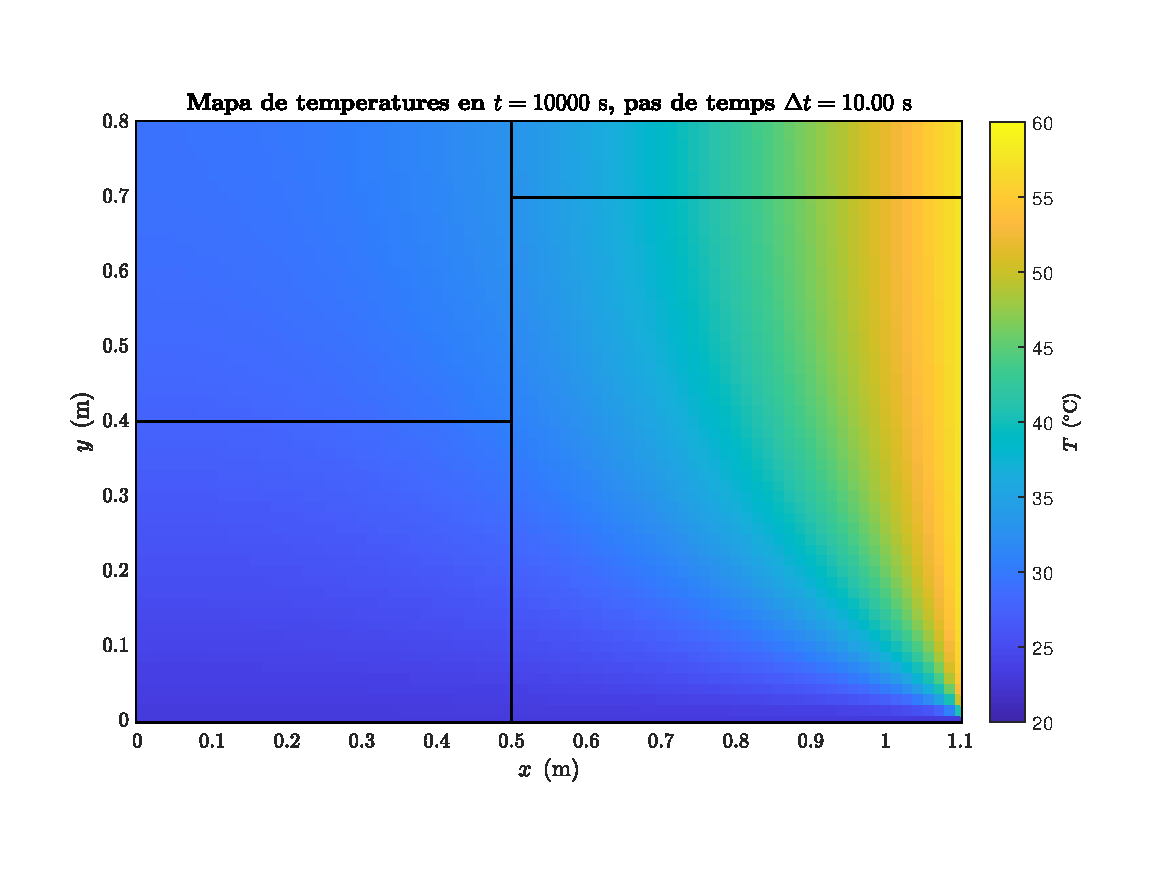
\includegraphics[width=.95\linewidth]{imagenes/04_influencia/pas_temps/pas_temps_16.pdf}
		\vspace{-15pt}
		\caption{Temps $t_\text{max} = 10000 \ \second$, pas de temps $\Delta t = 10.00 \ \second$.}
		\label{fig:pas_temps_16}
	\end{subfigure}
	\begin{subfigure}{.5\textwidth}
		\centering
		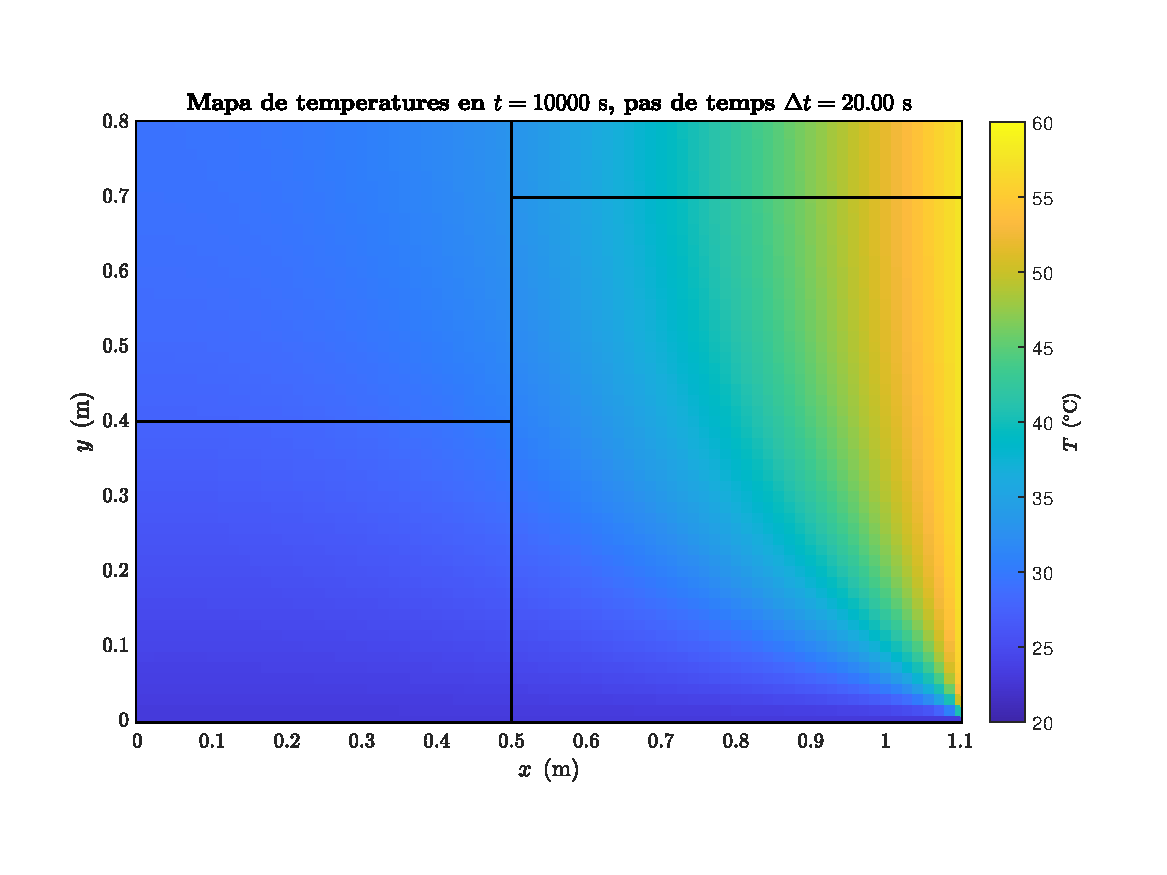
\includegraphics[width=.95\linewidth]{imagenes/04_influencia/pas_temps/pas_temps_17.pdf}
		\vspace{-15pt}
		\caption{Temps $t_\text{max} = 10000 \ \second$, pas de temps $\Delta t = 20.00 \ \second$.}
		\label{fig:pas_temps_17}
	\end{subfigure}%
	\begin{subfigure}{.5\textwidth}
		\centering
		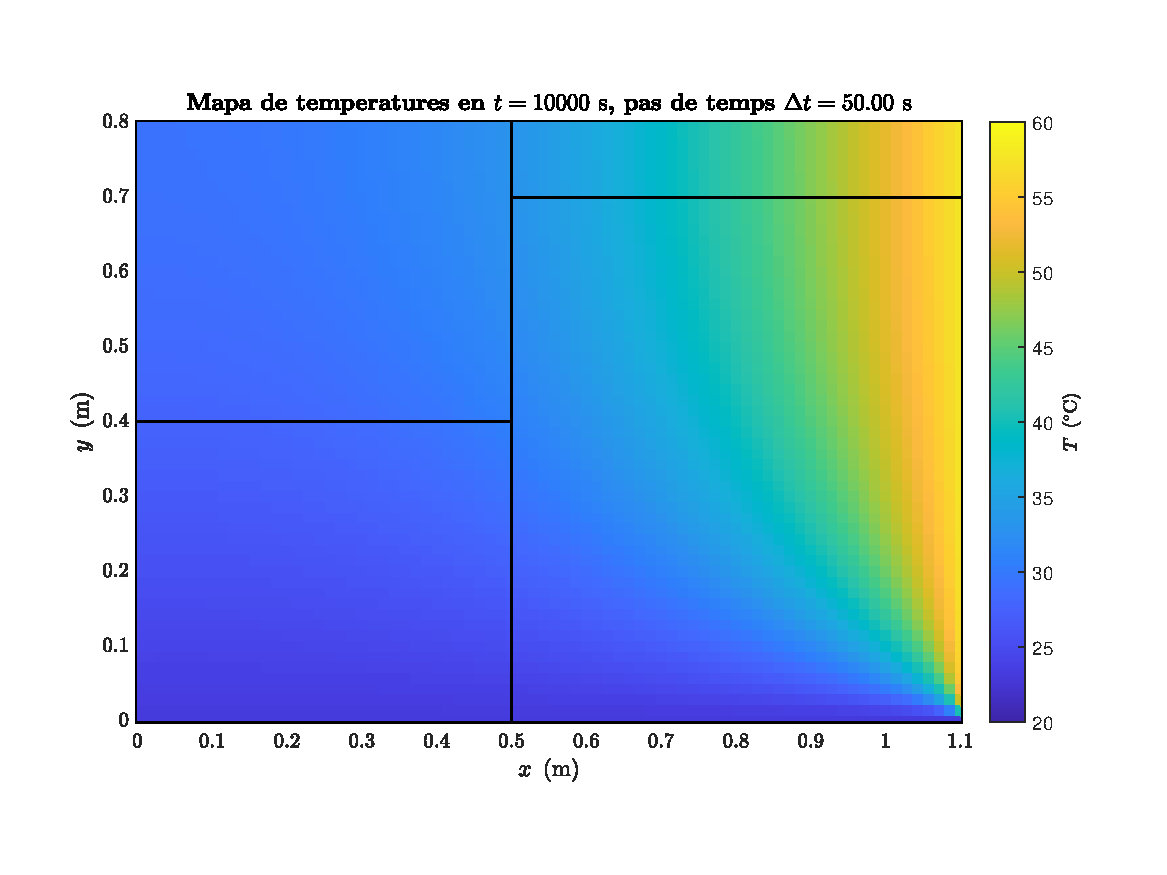
\includegraphics[width=.95\linewidth]{imagenes/04_influencia/pas_temps/pas_temps_18.pdf}
		\vspace{-15pt}
		\caption{Temps $t_\text{max} = 10000 \ \second$, pas de temps $\Delta t = 50.00 \ \second$.}
		\label{Temps fig:pas_temps_18}
	\end{subfigure}
	\caption{Mapes de temperatures en $t_\text{max} = 10000 \ \second$, discretització uniforme de $N_1 = 35$, amb passos de temps $\Delta = 0.50 \ \second, \, 1.00 \ \second, \, 5.00 \ \second, \, 10.00 \ \second, \, 20.00 \ \second$ i $50.00 \ \second,$, esquema de Crank--Nicolson i sense interpolació. L'escala de temperatures és entre $20 \ \celsius$ i $60 \ \celsius$. De nou s'observa que la zona de major gradient tèrmic és lleugerament més amplia amb $\Delta t$ petit. Els comentaris anteriors són aplicables en aquest cas.}	
	\label{fig:pas_temps_10000}
\end{figure} 